% Template for Cogsci submission with R Markdown

% Stuff changed from original Markdown PLOS Template
\documentclass[10pt, letterpaper]{article}

\usepackage{cogsci}
\usepackage{pslatex}
\usepackage{float}
\usepackage{caption}

% amsmath package, useful for mathematical formulas
\usepackage{amsmath}

% amssymb package, useful for mathematical symbols
\usepackage{amssymb}

% hyperref package, useful for hyperlinks
\usepackage{hyperref}

% graphicx package, useful for including eps and pdf graphics
% include graphics with the command \includegraphics
\usepackage{graphicx}

% Sweave(-like)
\usepackage{fancyvrb}
\DefineVerbatimEnvironment{Sinput}{Verbatim}{fontshape=sl}
\DefineVerbatimEnvironment{Soutput}{Verbatim}{}
\DefineVerbatimEnvironment{Scode}{Verbatim}{fontshape=sl}
\newenvironment{Schunk}{}{}
\DefineVerbatimEnvironment{Code}{Verbatim}{}
\DefineVerbatimEnvironment{CodeInput}{Verbatim}{fontshape=sl}
\DefineVerbatimEnvironment{CodeOutput}{Verbatim}{}
\newenvironment{CodeChunk}{}{}

% cite package, to clean up citations in the main text. Do not remove.
\usepackage{apacite}

% KM added 1/4/18 to allow control of blind submission


\usepackage{color}

% Use doublespacing - comment out for single spacing
%\usepackage{setspace}
%\doublespacing


% % Text layout
% \topmargin 0.0cm
% \oddsidemargin 0.5cm
% \evensidemargin 0.5cm
% \textwidth 16cm
% \textheight 21cm

\title{Re-examining cross-cultural similarity judgments using lexical
co-occurrence}

\usepackage[utf8]{inputenc}
\usepackage[T1, T2A, T5]{fontenc}
\usepackage{kotex}
\usepackage{booktabs}
\usepackage{longtable}
\usepackage{array}
\usepackage{multirow}
\usepackage{wrapfig}
\usepackage{float}
\usepackage{colortbl}
\usepackage{pdflscape}
\usepackage{tabu}
\usepackage{threeparttable}
\usepackage{threeparttablex}
\usepackage[normalem]{ulem}
\usepackage{makecell}
\usepackage{xcolor}

\author{{\large \bf Khuyen N. Le (knl005@ucsd.edu)}$^{1\star}$, {\large \bf Alexandra Carstensen (abc@ucsd.edu)}$^{1\star}$, \\ {\large \bf Shan Gao (shangaocog@gmail.com)$^2$} {\large \bf Michael C. Frank (mcfrank@stanford.edu)$^3$},  \AND $^1$Department of Psychology, UC San Diego, $^2$Department of Psychology, University of Chicago, \\ $^3$Department of Psychology, Stanford University }

\newlength{\cslhangindent}
\setlength{\cslhangindent}{1.5em}
\newenvironment{CSLReferences}%
  {}%
  {\par}

\begin{document}

\maketitle

\begin{abstract}
Is ``cow'' more closely related to ``grass'' or ``chicken''? Speakers of
different languages judge similarity in this context differently, but
why? One possibility is that cultures co-varying with these languages
induce differences in conceptualizations of similarity. Specifically,
East Asian cultures may promote reasoning about thematic similarity, by
which cow and grass are more related, whereas Western cultures may bias
judgments toward taxonomic relations, like cow-chicken. This difference
in notions of similarity is the consensus interpretation for
cross-cultural variation in this paradigm. We consider, and provide
evidence for, an alternative possibility, by which notions of similarity
are similar across contexts, but the statistics of the environment vary.
On this account, similarity judgments are guided by co-occurrence in
experience, and observing or hearing about cows and grass or cows and
chickens more often could induce preferences for these groupings, and
account in part for apparent differences in notions of similarity across
contexts.

\textbf{Keywords:}
similarity; culture; language; semantics; lexical co-occurrence;
variation
\end{abstract}

\hypertarget{introduction}{%
\section{Introduction}\label{introduction}}

\hypertarget{cross-cultural-variation-in-similarity}{%
\subsection{Cross-cultural variation in
similarity}\label{cross-cultural-variation-in-similarity}}

The way we partition our continuous experiences of the world into
categories, and which kind of similarity relationships we privilege to
organize such partitions, vary across cultures. One way this
cross-cultural difference has been observed is with a task comparing
preference for taxonomic and thematic similarity between East Asian and
Western participants.\footnote{Taxonomic categorization is based on the
  similarity of attributes, for example, similar perceptual properties,
  like shared color or shape, among objects.In contrast, thematic
  categorization is based on causal, spatial, and temporal relationships
  among objects (Markman \& Hutchinson, 1984).} Ji, Zhang, \& Nisbett
(2004) found that in a word triad task (choose two out of three words
that are more related to one another), Chinese participants preferred
thematic matching more compared to European Americans. In a pictorial
version of this task, Chiu (1972) found that Chinese children (9-10
years old) are also more likely to choose thematic matches compared to
their American counterparts. This cross-cultural difference is also
observed in novel object categorization, with Chinese participants
preferring to group by family resemblance across multiple features and
Americans preferring a single-feature rule (Norenzayan, Smith, Kim, \&
Nisbett, 2002).

Previous research has linked the observed difference in similarity
judgment to related work showing tendencies toward analytic processing
(emphasizing objects and their properties) in Western cultures and
holistic processing in East Asian cultures (emphasizing relationships
between objects and their context) (see also Nisbett (2003)).
Cross-cultural difference in similarity judgment is thus connected to
well-documented work showing East Asian participants exhibiting a higher
level of sensitivity to context than their Western counterparts when
reproducing drawings from memory (Ji, Peng, \& Nisbett, 2000); visually
exploring naturalistic scenes (Chua, Boland, \& Nisbett, 2005);
describing scenes (Masuda \& Nisbett, 2001); and in explaining the
causes of ambiguous behaviors (Choi, Nisbett, \& Norenzayan, 1999). This
view ascribes cross-cultural differences in similarity judgment to
variation in how each culture (or group of culture, i.e.~East Asian vs
Western) \textbf{conceptualize} similarity -- with East Asians
preferring thematic relations more than Westerners.

Alternatively, these judgments could be shaped by cross-cultural
differences in the \textbf{inputs} to similarity judgment, namely, the
statistics of the environment, and accordingly the content of everyday
experiences. Perhaps when faced with the triad task, participants from
all cultures follow the same process for conceptualizing similarity, but
rely on language or culture-specific inputs to this process. If we
observe a difference in categorization between East Asian and Western
participants, it could be that members of both groups use the same
procedure (considering similarity that is influenced by both taxonomic
and thematic relations), but the inputs to this procedure differ between
cultures, with East Asian participants exposed to more instances of
thematic similarity than their Western counterparts. We might also
expect that both conceptualization and inputs of similarity play a role
in driving cross-cultural differences -- East Asian participants may
both be exposed to more instances of thematic similarity, and prefer to
conceptualize similarity as thematic relations more so than Westerners.

\hypertarget{estimating-variation-in-experience}{%
\subsection{Estimating variation in
experience}\label{estimating-variation-in-experience}}

To test alternative hypotheses involving variation of inputs to
similarity judgment, we need a way to operationalize variation in
exposure to thematic vs taxonomic relations. While this metric is
difficult to directly measure, language statistics can provide a rough
proxy. Language statistics is useful in that it is part of the inputs to
everyday experiences (through spoken and written language), may afford
many of the `experiences' that people have with infrequently encountered
items, like cows or helicopters, and provides accessible measures.
Previous work also suggests that using language statistics (such as
lexical co-occurrence or cosine distance of word embeddings) as a proxy
can be a good predictor for similarity reasoning. Griffiths, Steyvers,
\& Tenenbaum (2007) showed that a model trained on word-document
co-occurrence can predict word association and the effects of semantic
association on a variety of linguistic tasks. Lexical semantic models
that are constructed using lexical co-occurrence (in comparison to
annotated relations) have been shown to perform well on predicting human
judgments about similarity between word pairs that are thematically or
taxonomically related (Rohde, Gonnerman, \& Plaut, 2006). Word
embeddings like fastText have been demonstrated to be good predictors
for similarity judgments (Liu, Feng, Wu, Chan, \& Fulton (2019),
Jatnika, Bijaksana, \& Suryani (2019)).

Our study uses cosine distances of fastText word vectors as a measure of
lexical co-occurrence\footnote{We also carried out our analysis using
  raw lexical co-occurrences and obtained similar results.}. fastText is
a system that uses lexical co-occurrence information to generate a
vector representing each word in its lexicon (Mikolov, Grave,
Bojanowski, Puhrsch, \& Joulin, 2018). fastText has also been shown to
be sensitive towards cultural effects on word meanings: Thompson \&
Lupyan (2020) showed that the distribution of semantic meaning clusters
generated by fastText trained on language-specific corpora correlates to
the cultural, historical and geographical distances of such languages
languages. This is a proof of concept for our use of fastText in
different languages with varying levels of relatedness.

We note that language statistics can incorporate both cultural-specific
environmental statistics (the inputs of similarity judgment) and
taxonomic/thematic preferences (the conceptualization of similarity).
For example, cultural features (farming) can lead to differences in
environmental statistics (seeing cows and grass) and in turn these can
influence language (talking more about cows and grass). But cultural
features (preferring thematic relations) could also more directly cause
individuals to talk differently about the same experiences (mentioning
what cows eat rather than what other animals cows are like). Therefore,
our approach looks at the extent to which language statistics can
predict cross-cultural differences in similarity judgment with the
understanding that language statistics is a proxy for both inputs and
conceptualization of similarity judgment\footnote{However, in Q3, we
  investigate whether differing culture-based conceptualization of
  similarity has unique contribution to cross-cultural variation of
  similarity jdugment.}.

\hypertarget{the-present-study}{%
\subsection{The present study}\label{the-present-study}}

Our study tests the hypothesis that, rather than (or in addition to) the
variation in conceptualization of similarity across cultural groups,
variation in the input to similarity judgment (namely, environmental
statistics as proxied by language statistics) can be used to predict
cross-cultural differences observed in how people evaluate similarity.
We note that our study is correlational and cannot make a causal claim
about the relationship of environmental statistics to similarity
judgment, but it may be possible to gain traction on potential
mechanisms by examining whether variation in similarity judgments covary
with environmental statistics that differ across cultural and linguistic
contexts. Our specific research questions are as follows:~

Q1: Do we replicate Ji et al. (2004) and extend the results to another
East Asian culture, namely Vietnam? Vietnam is a Southeast Asian country
that borders China and is historically greatly influenced by Chinese
culture (Hui, 2002). Therefore, it serves as a suitable cultural context
to investigate whether the claim made by Ji et al. (2004) and previous
studies, that Eastern and Western cultures have different notions of
similarity, extends beyond mainland China.

Q2: To what extent do cross-context environmental statistics (as proxied
by language) align with variation in similarity judgment?

Q3: Is there evidence for a unique contribution from conceptualization
of similarity?

Q4: Is language statistics viable as a standalone predictor, or is it
simply measuring conceptualization of similarity in a different way?~

To preview our results, we find that, while we do not find the predicted
Eastern/Western contrast in conceptualization of similarity in our
Vietnam extension, we do find that both language-specific statistics and
cultural contexts are a good predictor for cross-cultural differences in
similarity judgments. Language statistics are also a good predictor for
filler items with no taxonomic/thematic structure. Our findings are in
contrast to previous accounts, by which culture induces differing
conceptions of similarity (varying between taxonomic and thematic).
these findings provide an alternative, and more specific, account by
which language may explain these cross-cultural differences without
invoking variation in notions of similarity.

\hypertarget{methods}{%
\section{Methods}\label{methods}}

\hypertarget{participants}{%
\subsection{Participants}\label{participants}}

We recruited 200 participants from the US, 199 participants from
Vietnam, and 200 participants from mainland China. US participants were
recruited through snowball sampling seeded with Stanford student email
lists, Vietnam participants were recruited through snowball sampling
seeded with Vietnam-based student groups on Facebook, and mainland China
participants were recruited through snowball sampling seeded with group
chats on WeChat. US participants were compensated with \$5 gift
certificates (USD), VN participants received 50,000₫ (VND) in phone
credit, and mainland China participants received 25CNY through WeChat
credit transfer.

We excluded 8 US participants, 62 Vietnam participants, and 16 China
participants who missed 2 or more attention checks. We followed 4
exclusion criteria that aim to retain only participants who are
influenced by one culture: (1) non-native speakers of English and
Vietnamese, respectively, (2) fluent in at least one of the other two
study languages (Vietnamese for US participants, English for Vietnamese
participants and Chinese participants), (3) have lived outside of the
test country (US, Vietnam, or China) for more than two years, and (4)
have significant international experience (more than 6 international
experiences of 2 days or longer.) We did not use a particular criterion
for a language if it would exclude 25\% or more of any one sample. In
this round of exclusion, we excluded 73 US, 27 Vietnam participants, and
35 China participants. After these exclusions, the US sample included
119 participants (30M, 84F, 3 non-binary, 2 other), with mean age = 22.2
(SD = 8.15) and median age = 20. The Vietnam sample included 110
participants (34M, 71F, 5 other), with mean age = 22.21 (SD = 5.81) and
median age = 21. The China sample included 149 participants (61M, 87F, 1
other), with mean age = 23.1 (SD = 3.65) and median age = 23.\footnote{A
  table summarizing number of participants lost at each round of
  exclusions is included in the Supplementary Information.}

We preregistered a more stringent exclusion criterion where participants
were excluded if they missed any attention checks. However, this led to
a small sample size, especially for Vietnam context (US = 109, China =
132, Vietnam = 57). Our reported results with the less stringent
exclusion criterion (detailed above) is largely not different from the
results with the preregistered criterion. Any differences are noted in
the Analysis section.

\hypertarget{stimuli-materials}{%
\subsection{Stimuli Materials}\label{stimuli-materials}}

We adapted stimuli from previous studies to create a set of test triads
consisting of a cue, with one thematic and one taxonomic match option.
For example, ``cow,'' ``grass,'' and ``chicken,'' where ``cow'' is the
cue, ``grass'' is the thematic match, and ``chicken'' the taxonomic
match. We included 105 such triads, a superset including triads pulled
from supplemental information and in-text examples across the
literature, and others that we adapted or created . We selected triads
on the basis of cultural familiarity in the US, Vietnam, and China. The
triads were originally in English; they were translated to Vietnamese
and Mandarin by a fluent bilingual speaker in each language. The
translations were then checked for accuracy after backtranslation to
English by another fluent bilingual in each language who was naive to
the original English versions. All materials are included in the
Supplementary Information.

\hypertarget{procedure}{%
\subsection{Procedure}\label{procedure}}

Each participant completed all 105 triads in sets of 21 trials at a time
(10 test triads, 10 filler triads, and 1 attention check per page), by
selecting the match most related to the cue (``Which thing is most
closely related to the bolded item?'' and translated equivalents). The
test triads were presented with 105 filler triads mixed in, to obscure
the taxonomic-thematic two-answer forced choice structure of the test
stimuli and reduce the likelihood that participants would become aware
of the design. The filler triads were groups of three semantically
related words, but where the match options were not distinguished by
thematic vs.~taxonomic similarity, e.g., cue ``bird'' with match options
``lizard'' and ``toad.'' Additionally, we included 10 attention check
trials, which were formatted like the test and filler triads but
included an instruction instead of a cue item, e.g., ``Choose wife''
with match options ``wife'' and ``husband.'' In total, each participant
completed 210 similarity judgments and 10 attention check questions,
with triads presented in randomized orders that varied between subjects.

\hypertarget{corpus-model}{%
\subsection{Corpus model}\label{corpus-model}}

Our general approach is to predict behavioral preferences in similarity
judgment using relative similarity between word embeddings.

\hypertarget{word-vector-retrieval}{%
\paragraph{Word vector retrieval}\label{word-vector-retrieval}}

We use the fastText pre-trained models of English, Mandarin, and
Vietnamese in Grave, Bojanowski, Gupta, Joulin, \& Mikolov (2018). These
models are trained on Common Crawl and Wikipedia using We distribute
pre-trained word vectors for 157 languages, trained on Common Crawl and
Wikipedia using fastText. These models were trained using a Continuous
Bag of Words (CBOW) with position-weights and a window of size 5. The
models use character n-grams of length 5 and 10 negative examples. From
the aforementioned models, we retrieve the word vectors (dimension 300)
for each word we are interested in.

\hypertarget{similarity-model}{%
\paragraph{Similarity model}\label{similarity-model}}

To give an intuition for our model, consider again the cow-grass-chicken
triad: we retrieved word vectors for ``cow'' and ``grass'', and
calculate the cosine distance between these vectors. Similarly, we
retrieved vectors for ``cow'' and ``chicken'' and calculate the cosine
distance between them. Our similarity prediction is then inversely
proportional to the ratio of cosine distance of these pairs. This is
because a larger cosine distance means the word vectors are further
apart, and thus the words are less similar. For example, if the cosine
distance of thematic cow-grass is 0.7 and the cosine distance of
taxonomic cow-chicken is 0.3, then our model predicts, correspondingly,
that 30\% of responses to the triad will be grass, and the other 70\%
chicken.

In practice, we calculated the cosine distance between each cue-thematic
match (thematic cosine distance) and cue-taxonomic match (taxonomic
cosine distance), using the spatial.distance.cosine function from the
SciPy package (Virtanen et al., 2020). We then calculated the thematic
cosine distance proportion as thematic cosine distance over the sum of
taxonomic cosine distance and thematic cosine distance. We did this for
all three corpora. We were able to obtain predictions for all triads in
all languages. We then use a mixed-effects regression to evaluate how
well each corpus model predicts participants' similarity judgments,
across triads and cultural contexts.

\hypertarget{results}{%
\section{Results}\label{results}}

\hypertarget{replication-of-previous-work-and-extension-to-a-vietnamese-sample}{%
\subsection{1. Replication of previous work and extension to a
Vietnamese
sample}\label{replication-of-previous-work-and-extension-to-a-vietnamese-sample}}

Following previous work, we would expect participants from mainland
China to prefer thematic matches more than US participants (to use the
cow-grass-chicken triad: we would expect participants from mainland
China to prefer the cow-grass match over the cow-chicken match to a
larger extent compared to US participants). We would also expect that
participants from Vietnam would pattern with China, and also show a
significantly higher preference for thematic matches compare to US
participants.

The group means of proportion of thematic response in mainland China is
the highest (M = 0.65, SD = 0.11), followed by the groups means in
Vietnam (M = 0.6, SD = 0.11), which is slightly higher than that of the
US (M = 0.56, SD = 0.17) (Figure 1).

\begin{CodeChunk}
\begin{figure}[tb]

{\centering 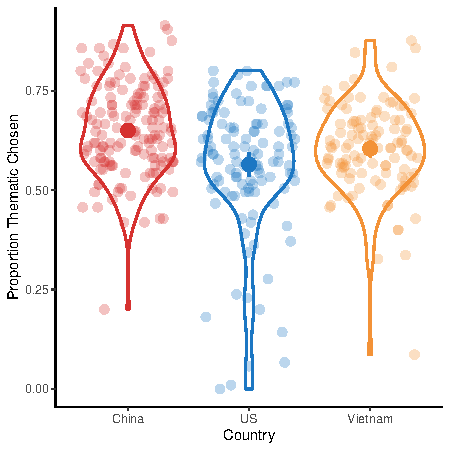
\includegraphics{figs/unnamed-chunk-1-1} 

}

\caption[Proportion of thematic responses by country]{Proportion of thematic responses by country.}\label{fig:unnamed-chunk-1}
\end{figure}
\end{CodeChunk}

To test for cross-context differences in similarity judgments between
the countries, we ran a mixed-effects logistic regression predicting
triad responding (taxonomic or thematic) with country (US, China, or
Vietnam) as a fixed effect. As random effects, we included an intercept
per subject and one per triad, as well as by-triad random slopes for
country to account for variation in the country effect across triads.

Overall, there is a significant effect of country on proportion of
thematic responses (\(\chi^2\)(2) = 15.37, p \textless{} .001). However,
this effect is driven by the difference between US and China responding
(\(\beta\) = -0.48, p \textless{} .001). There is no statistical
difference between the Vietnam and China responding (\(\beta\) = -0.22,
p = 0.09), and the US and Vietnam responding (\(\beta\) = 0.26, p =
0.086).

On this analysis, we do not find support that the US-China tendencies
toward taxonomic and thematic responding (respectively) extend to the
US-Vietnam comparison. Accordingly, we cannot speak to overall biases
toward thematic responding across Asian cultural contexts broadly, but
we do replicate the differences documented by Ji et al. (2004) between
the US and China. However, in our corpus model comparison, we do find
evidence for different, more fine-grained variation in similarity
judgments between the US and Vietnam.

\hypertarget{language-statistics-as-a-predictor-for-cross-cultural-variation-in-similarity-judgments}{%
\subsection{2. Language statistics as a predictor for cross-cultural
variation in similarity
judgments}\label{language-statistics-as-a-predictor-for-cross-cultural-variation-in-similarity-judgments}}

\hypertarget{single-corpus-model}{%
\subsubsection{Single corpus model}\label{single-corpus-model}}

To test whether variation in language statistics can explain differences
in similarity judgments between US and Vietnam participants, we compare
logistic mixed-effects regression models fit to the thematic responding
data from each country separately. We first ask how well each corpus
model (English, Vietnamese, or Mandarin) predicts similarity judgments
by speakers of the corresponding language (US, Vietnam, or China). To do
this, we use a mixed-effects logistic regression to predict triad
responses (0=taxonomic or 1=thematic) with corpus prediction (proportion
of cosine distance) as a fixed effect and participant and triad as
random effects. If environmental statistics (as proxied by language
statistics) contribute to the differences in similarity judgments, we
would expect each language corpus to be a good predictor for similarity
judgment responding in its corresponding context.

We found that all corpora are significant predictors of all cultural
context responding, with p \textless{} 0.05 and \(\beta\) from -8.69 to
-2.4. (For a full report, see Supplementary Information.)

While each corpus is a good predictor for its corresponding context, the
fact that all corpora covary with all cultural contexts suggests that
language is such a rich proxy of human experience that even using the
wrong proxy (e.g.~Mandarin for US responding) is informative. A single
corpus model might therefore not be informative in culture-specific
ways, but might only reflect consistency in experiences across cultures.

\hypertarget{multiple-corpora-model}{%
\subsubsection{Multiple corpora model}\label{multiple-corpora-model}}

If language statistics is able to predict meaningful culture-specific
variation in similarity judgment (rather than just consistency across
cultures), we would expect each corpus to be the best predictor of its
corresponding culture compared to the other two corpora. We directly
compare the corpus models by including both as fixed effects in three
mixed-effect regressions (predicting US, Vietnam and China responding)
with the same random effects as above.

For US responding: only the English (EN) corpus is a significant
predictor\footnote{With preregistered exclusion criterion: only the
  English (EN) and Mandarin (ZH) corpus are significant predictors.}. EN
corpus: \(\beta\) = -6.96, \(\chi^2\)(1) = 16.57, p \textless{} .001. VI
corpus: \(\beta\) = -2.22, \(\chi^2\)(1) = 3.73, p = 0.054. ZH corpus:
\(\beta\) = -3.18, \(\chi^2\)(1) = 3.37, p = 0.066.

For Vietnam responding: only the Vietnamese (VI) and Mandarin (ZH)
corpus are significant predictors\footnote{With preregistered exclusion
  criterion: all three corpora are significant predictors.}. EN corpus:
\(\beta\) = -2.98, \(\chi^2\)(1) = 2.58, p = 0.108. VI corpus: \(\beta\)
= -2.75, \(\chi^2\)(1) = 4.84, p = 0.028. ZH corpus: \(\beta\) = -4.39,
\(\chi^2\)(1) = 5.49, p = 0.019.

For China responding: only the Mandarin (ZH) and English (EN) corpus are
significant predictors. EN corpus: \(\beta\) = -3.32, \(\chi^2\)(1) =
7.18, p = 0.007. VI corpus: \(\beta\) = -1.59, \(\chi^2\)(1) = 3.63, p =
0.057. ZH corpus: \(\beta\) = -5.31, \(\chi^2\)(1) = 17.69, p
\textless{} .001.

We observed some level of language specificity from this analysis. The
English corpus is the best predictor for US responding, and the Mandarin
corpus is the best predictor for China response. While this is not the
case with the Vietnamese corpus and the Vietnam responding, the
Vietnamese corpus is still a significant predictor for the Vietnam
responding (Figure 2). These results strengthens our hypothesis that
variation in inputs to similarity judgment (as proxied by language
statistics) can predict cross-cultural variations of similarity
judgment.

\begin{CodeChunk}
\begin{figure}[tb]

{\centering 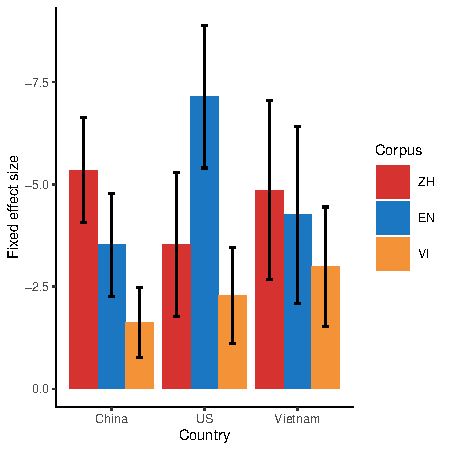
\includegraphics{figs/unnamed-chunk-3-1} 

}

\caption[Fixed effect sizes of each corpus lexical statistics (cosine distance proportion) when included as a predictor for China, US, and Vietnam responding, respectively]{Fixed effect sizes of each corpus lexical statistics (cosine distance proportion) when included as a predictor for China, US, and Vietnam responding, respectively. The English corpus is the best predictor for US response, and the Mandarin corpus is the best predictor for China response.}\label{fig:unnamed-chunk-3}
\end{figure}
\end{CodeChunk}

However, in all cultural contexts, adding the other two corpora produces
a significantly better fit than the identical model without the
additional corpora, and only the corresponding corpus included as a
predictor (US response: \(\chi^2\)(2) = 7.93, p = 0.019; Vietnam
response: \(\chi^2\)(2) = 13.72, p = 0.001; China response:
\(\chi^2\)(2) = 10.56, p = 0.005). This analysis suggests that
culture-specific inputs to similarity judgment (as proxied by language
statistics) do not fully explain cross-cultural differences in
similarity judgment.

\hypertarget{cultural-context-as-a-predictor-for-cross-cultural-variation-in-similarity-judgments}{%
\subsection{3. Cultural context as a predictor for cross-cultural
variation in similarity
judgments}\label{cultural-context-as-a-predictor-for-cross-cultural-variation-in-similarity-judgments}}

Our above models tested whether language statistics is a good predictor
for similarity judgment. As we noted above, language statistics can be a
proxy of both inputs and conceptualization of similarity. However, it is
still an open question whether conceptualization of similarity itself
has a unique contribution to similarity judgment (beyond its influence
on language statistics). To test this hypothesis, we operationalize
cultural-specific conceptualization of similarity as country. We then
compare a model that includes country, corresponding corpus statistics
and their interaction as fixed effects to a model with only the
corresponding corpus statistics as the fixed effect. If
conceptualization of similarity has a unique contribution to similarity
judgment, we should see that terms including country to be a significant
predictor of responding.

In the model containing only the corresponding corpus statistics, the
corpus statistics is a significant predictor (\(\beta\) = -1.79,
\(\chi^2\)(1) = 75.58, p \textless{} .001). When adding country and
interaction between country and corpus, corpus statistics (\(\beta\) =
-1.72, \(\chi^2\)(1) = 23.34, p \textless{} .001), country (F(2,
\ensuremath{\infty{}}) = 13.18, \(\chi^2\)(2) = 7.39, p = 0.025), and
interaction between country and corpus (F(2, \ensuremath{\infty{}}) =
6.66, \(\chi^2\)(2) = 13.33, p = 0.001), are significant
predictors\footnote{With preregistered exclusion criterion: only corpus
  statistics and interaction between country and corpus are significant
  predictors.}. Including the country and country-corpus terms to the
language-only model significantly its ability to explain variation in
responding (\(\chi^2\)(4) = 40.76, p \textless{} .001). This result
points to a unique contribution by culture-specific ways of
conceptualizing similarity to similarity judgment that is not captured
in language statistics.

\hypertarget{language-statistics-as-a-predictor-for-non-structured-triad-items}{%
\subsection{4. Language statistics as a predictor for non-structured
triad
items}\label{language-statistics-as-a-predictor-for-non-structured-triad-items}}

A possible concern with our approach is that variation in language
statistics (which we claim to be a proxy of both inputs and
conceptualization of similarity) can be fully explained by variation in
conceptualization of similarity (i.e.~the difference in similarity
measures between `cow' and `grass' versus `cow' and `chicken' in one
corpus is solely driven by the corresponding culture's preference of
thematic versus taxonomic categorization). Alternatively, language
statistics may be measuring slight but pervasive differences in
similarity driven by participants' different cultural contexts, rather
than merely the type of similarity they generally prefer (thematic vs
taxonomic relations). We address this concern by testing whether
language statistics covary with similarity judgment of items with no
taxonomic/thematic structures (filler items). If language statistics is
only driven by conceptualization of similarity, we should not see an
effect with such items, which have no structured similarity relations by
which to make any predictions.~

\begin{CodeChunk}
\begin{figure}[tb]

{\centering 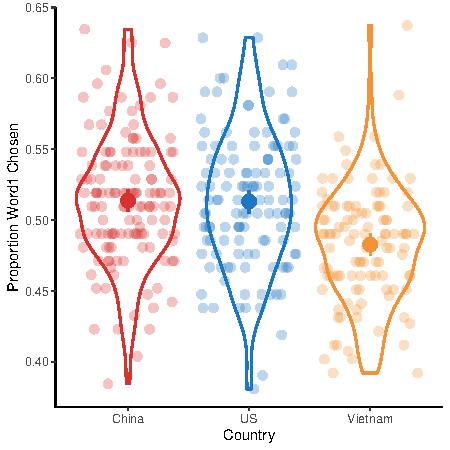
\includegraphics{figs/unnamed-chunk-4-1} 

}

\caption[Proportion of Word1 responses by country]{Proportion of Word1 responses by country.}\label{fig:unnamed-chunk-4}
\end{figure}
\end{CodeChunk}

For each filler triad, we randomly assigned one of the responding
options as `Word1'. Running a mixed-effects logistic regression to
predict responding (Word1 or Word2) with country as the fixed effect and
a random effect structure equivalent to Q1, we found no effect of
country on filler responding (\(\chi^2\)(2) = 0.74, p = 0.692) (Figure
3).

Using the same mixed-effects logistic regression structure as Q2, we
predict responses (1=word1 or 0=word2) of each cultural context with the
corresponding corpus statistics as a fixed effect, and participant and
triad as random effects. We found that in all cultural contexts, the
corresponding corpus is a significant predictor of responding, with p
\textless{} 0.05 and \(\beta\) from -9.59 to -3.14. (For a full report,
see Supplementary Information.)

\hypertarget{discussion}{%
\section{Discussion}\label{discussion}}

In this paper, we consider whether statistics of the environment (as
proxied by langauge statistics) can account for cross-cultural
differences in a classic similarity judgment paradigm, as an alternative
to the view that members of different cultures vary in their
conceptualization of similarity. While we managed to replicate the
previously documented contrast between English speakers in the US and
Mandarin Chinese speakers from East Asia (mainland China, Taiwan, Hong
Kong, and Singapore), we do not extend this contrast to our sample of
Vietnamese speakers in Vietnam and English speakers in the US. This
finding suggests some limitations on the generality of the cultural
account. We found some support for the environmental statistics account:
each corpus statistics is a good predictor for the corresponding
country's similarity judgments, even when other corpus statistics are
included, and even with triads without a taxonomic/thematic structure.
However, we also found that culture-based conceptualization of
similarity uniquely contributes to predicting similarity judgment when
included in a model with corpus statistics. Overall, our results provide
evidence that cross-cultural differences in similarity judgment might
not be driven by cross-cultural differences in conception of similarity
alone, but also by variation in inputs to similarity judgment.

There are some important limitations of our approach. While we discuss
cross-cultural variability at the level of countries or larger world
areas, these are not cultural monoliths. For convenience, we
operationalize culture at the level of country, based on where
participants were raised. It is an open question whether performance in
our participant populations (of relatively young and well-educated
adults) is representative of the broader country. This is especially
true for societies with substantial ethnic and cultural variation such
as the US. We expect that our data is likely to underestimate variation
both within and between the countries we sample from.

Additionally, language, culture, cognition, and individual experiences
are intertwined in complex causal relationships. In this study, we
measure language and its relation to cross-cultural differences in
categorization, but these relations test only the plausibility of a
language-based account; they cannot establish the direction of
causality.

Our findings raise additional questions for future work: To what extent
are the relativity effects driven by language, and to what extent by
culture? Ji et al. (2004) established that culture-aligned differences
in this paradigm exist, even when the test language is held constant,
concluding that ``it is culture (independent of the testing language)
that led to different grouping styles'' in their study. Our data provide
a cautionary note to this conclusion, suggesting that semantic
representations in bilinguals (see Francis (2005) for a review) may have
the potential to provide an offline account for cross-context
differences in similarity judgments, independent of test language.
However, there are still many open questions for this account. How do
semantic associations guide categorization? Can they explain
taxonomic-thematic differences of the type reported by Ji et al. (2004)
and others? Can we provide a more specific computational account than
the simple proportion-of-similarity model tested here?

Despite these caveats, our findings here demonstrate the plausibility of
an alternative perspective on cross-cultural accounts of language,
thought, and similarity in the case of taxonomic and thematic reasoning:
that it may be the input to similarity judgments, rather than the
evaluative process or the conceptualization of similarity that produces
variation in similarity reasoning across cultural and linguistic
contexts. We hope this work provides a foundation for further research
probing this question.

\hypertarget{acknowledgements}{%
\section{Acknowledgements}\label{acknowledgements}}

Place acknowledgments (including funding information) in a section at
the end of the paper.

\hypertarget{references}{%
\section{References}\label{references}}

\setlength{\parindent}{-0.1in} 
\setlength{\leftskip}{0.125in}

\noindent

\newpage

\hypertarget{refs}{}
\begin{CSLReferences}{1}{0}
\leavevmode\vadjust pre{\hypertarget{ref-Chiu1972}{}}%
Chiu, L. (1972). A cross-cultural comparison of cognitive styles in
chinese and american children. \emph{International Journal of
Psychology}, \emph{7}(4), 235--242.
http://doi.org/\href{https://doi.org/doi:10.1080/00207597208246604}{doi:10.1080/00207597208246604}

\leavevmode\vadjust pre{\hypertarget{ref-Choi1999}{}}%
Choi, I., Nisbett, R. E., \& Norenzayan, A. (1999). Causal attribution
across cultures: Variation and universality. \emph{International Journal
of Psychology}, \emph{125}(1), 47--63.
http://doi.org/\href{https://doi.org/doi:10.1037/0033-2909.125.1.47}{doi:10.1037/0033-2909.125.1.47}

\leavevmode\vadjust pre{\hypertarget{ref-Chua2005}{}}%
Chua, H. F., Boland, J. E., \& Nisbett, R. E. (2005). Cultural variation
in eye movements during scene perception. \emph{Proceedings of the
National Academy of Sciences}, \emph{102}(35), 12629--12633.
http://doi.org/\href{https://doi.org/10.1073/pnas.0506162102}{10.1073/pnas.0506162102}

\leavevmode\vadjust pre{\hypertarget{ref-Francis2005}{}}%
Francis, W. S. (2005). \emph{Bilingual semantic and conceptual
representation}. Oxford University Press.

\leavevmode\vadjust pre{\hypertarget{ref-Grave2018}{}}%
Grave, E., Bojanowski, P., Gupta, P., Joulin, A., \& Mikolov, T. (2018).
Learning word vectors for 157 languages. In \emph{Proceedings of the
international conference on language resources and evaluation (LREC
2018)}.

\leavevmode\vadjust pre{\hypertarget{ref-Griffiths2007}{}}%
Griffiths, T. L., Steyvers, M., \& Tenenbaum, J. B. (2007). Topics in
semantic representation. \emph{Psychological Review}, \emph{114}(2),
211--244.
http://doi.org/\href{https://doi.org/doi:10.1037/0033-295x.114.2.211}{doi:10.1037/0033-295x.114.2.211}

\leavevmode\vadjust pre{\hypertarget{ref-Hui2002}{}}%
Hui, W. (2002). Modernity and 'asia' in the study of chinese history. In
E. Fuchs \& B. Stuchteyi (Eds.), \emph{Across cultural borders:
Historiography in global perspective}. Rowman \& Littlefield.

\leavevmode\vadjust pre{\hypertarget{ref-Jatnika2019}{}}%
Jatnika, D., Bijaksana, M. A., \& Suryani, A. A. (2019). Word2Vec model
analysis for semantic similarities in english words. \emph{Procedia
Computer Science}, \emph{157}, 160--167.
http://doi.org/\url{https://doi.org/10.1016/j.procs.2019.08.153}

\leavevmode\vadjust pre{\hypertarget{ref-Ji2000}{}}%
Ji, L., Peng, K., \& Nisbett, R. E. (2000). Culture, control, and
perception of relationships in the environment. \emph{Journal of
Personality and Social Psychology}, \emph{78}(5), 943--955.
http://doi.org/\href{https://doi.org/doi:10.1037/0022-3514.78.5.943}{doi:10.1037/0022-3514.78.5.943}

\leavevmode\vadjust pre{\hypertarget{ref-Ji2004}{}}%
Ji, L., Zhang, Z., \& Nisbett, R. E. (2004). Is it culture or is it
language? Examination of language effects in cross-cultural research on
categorization. \emph{Journal of Personality and Social Psychology},
\emph{87}(1), 57--65.
http://doi.org/\href{https://doi.org/doi:10.1037/0022-3514.87.1.57}{doi:10.1037/0022-3514.87.1.57}

\leavevmode\vadjust pre{\hypertarget{ref-Liu2019}{}}%
Liu, N., Feng, C., Wu, S., Chan, A., \& Fulton, J. (2019). Automate RFP
response generation process using FastText word embeddings and soft
cosine measure. In \emph{Proceedings of the 2019 international
conference on artificial intelligence and computer science} (pp.
12--17).
http://doi.org/\href{https://doi.org/10.1145/3349341.3349362}{10.1145/3349341.3349362}

\leavevmode\vadjust pre{\hypertarget{ref-Markman1984}{}}%
Markman, E. M., \& Hutchinson, J. E. (1984). Children's sensitivity to
constraints on word meaning: Taxonomic versus thematic relations.
\emph{Cognitive Psychology}, \emph{16}(1), 1--27.
http://doi.org/\href{https://doi.org/doi:10.1016/0010-0285(84)90002-1}{doi:10.1016/0010-0285(84)90002-1}

\leavevmode\vadjust pre{\hypertarget{ref-Masuda2001}{}}%
Masuda, T., \& Nisbett, R. E. (2001). Attending holistically versus
analytically: Comparing the context sensitivity of japanese and
americans. \emph{Journal of Personality and Social Psychology},
\emph{81}(5), 922--934.
http://doi.org/\href{https://doi.org/doi:10.1037/0022-3514.81.5.922}{doi:10.1037/0022-3514.81.5.922}

\leavevmode\vadjust pre{\hypertarget{ref-Mikolov2018}{}}%
Mikolov, T., Grave, E., Bojanowski, P., Puhrsch, C., \& Joulin, A.
(2018). Advances in pre-training distributed word representations. In
\emph{Proceedings of the international conference on language resources
and evaluation (LREC 2018)}.

\leavevmode\vadjust pre{\hypertarget{ref-Nisbett2003}{}}%
Nisbett, R. E. (2003). \emph{The geography of thought: How asians and
westerners think differently \ldots{} and why}. New York: Free Press.

\leavevmode\vadjust pre{\hypertarget{ref-Norenzayan2002}{}}%
Norenzayan, A., Smith, E. E., Kim, B. J., \& Nisbett, R. E. (2002).
Cultural preferences for formal versus intuitive reasoning.
\emph{Cognitive Science}, \emph{26}(5), 653--684.
http://doi.org/\href{https://doi.org/doi:10.1207/s15516709cog2605_4}{doi:10.1207/s15516709cog2605\_4}

\leavevmode\vadjust pre{\hypertarget{ref-Rohde2006}{}}%
Rohde, D. L., Gonnerman, L. M., \& Plaut, D. C. (2006). An improved
model of semantic similarity based on lexical co‐occurrence.
\emph{Communications of the ACM}, \emph{8}, 627--633.

\leavevmode\vadjust pre{\hypertarget{ref-Thompson2020}{}}%
Thompson, R., B., \& Lupyan, G. (2020). Cultural influences on word
meanings revealed through large-scale semantic alignment. \emph{Nature
Human Behaviour Volume}, \emph{4}, 1029--1038.
http://doi.org/\url{https://doi.org/10.1038/s41562-020-0924-8}

\leavevmode\vadjust pre{\hypertarget{ref-2020SciPy}{}}%
Virtanen, P., Gommers, R., Oliphant, T. E., Haberland, M., Reddy, T.,
Cournapeau, D., \ldots{} SciPy 1.0 Contributors. (2020). {{SciPy} 1.0:
Fundamental Algorithms for Scientific Computing in Python}. \emph{Nature
Methods}, \emph{17}, 261--272.
http://doi.org/\href{https://doi.org/10.1038/s41592-019-0686-2}{10.1038/s41592-019-0686-2}

\end{CSLReferences}

\bibliographystyle{apacite}


\end{document}
